\documentclass[a4paper,12pt,abstracton]{scrartcl}
\usepackage[ngerman, english]{babel}
\usepackage[utf8]{inputenc}
\usepackage[T1]{fontenc}
\usepackage{graphicx}
\usepackage{lipsum}
\usepackage{blindtext}
\usepackage{color}
\usepackage{setspace}
\usepackage{hyperref}
\usepackage[printonlyused]{acronym}
\usepackage{amsmath}
\usepackage{amsfonts}
\usepackage{amssymb}
\usepackage[export]{adjustbox}
\usepackage{subcaption}
\usepackage{makecell}
\usepackage[]{units}
\usepackage{natbib}
\usepackage{aas_macros}
\usepackage{enumerate}


\title{Bachelorarbeit}
\author{Sophia Milanov}
\date{\today}

\begin{document}
\bibliographystyle{glenn} 
\pagenumbering{roman}

\onehalfspacing
\begin{titlepage}
\begin{center}
 
\Large\textbf{Department of Physics and Astronomy\\
University of Heidelberg}

\vspace{16cm}

\normalsize
Bachelor Thesis in Physics\\
submitted by \\
\vspace{0.5cm}
\Large\textbf{Sophia Milanov}\\
\normalsize
\vspace{0.5cm}
born in Düsseldorf (Germany)\\
\vspace{0.5cm}
\Large\textbf{2016}
\normalsize

\newpage




\Large\textbf{Title}

\vspace{18cm}

\normalsize
This Bachelor Thesis has been carried out by Sophia Milanov at the\\
Max Planck Institute for Astronomy in Heidelberg\\
under the supervision of\\
Dr. Glenn van de Ven

\vfill
\end{center}

\end{titlepage}


\begin{abstract}
\blindtext 
\end{abstract}

\newpage
\addtocontents{toc}{\protect\enlargethispage{2\baselineskip}}
\tableofcontents

\newpage
\pagenumbering{arabic}



\section{Introduction}\label{Introduction}
Globular clusters (\acsp{GC})\acused{GC} are self-gravitating, gas-free systems of maybe 10\(^5\) to maybe 10\(^7\) stars which are spherically grouped. There are about 150 of them in the \ac{MW}. Since they are some of the oldest stellar populations in the universe (approximately 13 Gyr), they contain much information about the assembly history and evolution of the \ac{MW}. Formerly seen as very simple spherical and isotropic stellar systems with only one stellar population, recent research revealed a much higher degree of complexity (that differ in the light-elements abundances). \acp{GC} are now known to host multiple stellar populations that challenge our understanding of their formation. Moreover, \acp{GC} now also appear dynamically complex, presenting deviations from spherical symmetry, anisotropy in velocity space and significant internal rotation.
 
\par Recent attention has been devoted to the search of \acp{IMBH} in the centre of \acp{GC}. These elusive black holes \(10^3 \mathrm{M}_\odot < \mathrm{M}_\bullet < 10^4 \mathrm{M}_\odot\) could be the missing link between stellar mass black holes (\(\mathrm{M}_\bullet < 100 \mathrm{M}_\odot\)) and super massive black holes (\acsp{SMBH}, \(\mathrm{M}_\bullet > 10^5 \mathrm{M}_\odot\))\acused{SMBH} as they could represent the seed for the formation of \acp{SMBH}. Their search in the centre of \acp{GC} has partially been motivated by the extrapolation of the \(\mathrm{M}_\bullet-\sigma\)-relation for galaxies, describing the relation between the mass of a central massive black hole and the velocity dispersion of its host galaxy.
\par The hunt of \acp{IMBH} in Galactic \acp{GC} has been primarily based on two methods: 1) detection of radio and X-ray emission due to the accretion of gas in the black hole; 2) detection of kinematic signatures in the central region of a \ac{GC}. The first method proved to be difficult because the feeding of a black hole with gas is highly inefficient in a gas poor environment of Galactic \acp{GC}. 
\par The kinematic detection of \acp{IMBH} is usually based on the analysis of the velocity-dispersion profile in the inner few arcseconds around the crowded centre of a \ac{GC} in search for a rise of the dispersion. This requires a combination of high angular resolution and high spectral resolving power. For this reason the detection of \acp{IMBH} remains still highly controversial. 
\par Currently there are two different kinematic methods trying to detect \acp{IMBH}: \color{red} resolved kinematics \& unresolved integrated light [bianchini 2015] \cite{2015MNRAS.453..365B} \color{black} These methods often deliver significant different results when applied to the same \ac{GC}. As an example there are the unresolved/integrated IFU kinematics which result in a signature of an \ac{IMBH} for NGC 6388 (cusp in the velocity dispersion profile) and resolved/discrete kinematics which do not yield \acp{IMBH} (no cusp in the velocity dispersion profile). 
\begin{figure}
\centering
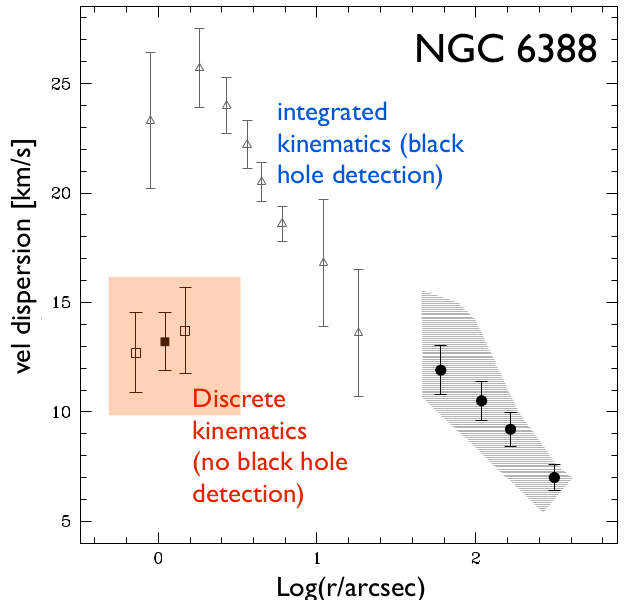
\includegraphics[width=0.5\textwidth]{/home/sophia/Paolo_talk_plot.png}
\caption{Velocity profile of NGC 6388 derived by the two different methods. We see a cusp given by the integrated kinematics method while there is no cusp with discrete kinematics. \citep{2013ApJ...769..107L} \color{red}and bianchini?\color{black}}
\label{fig:NGC6388}
\end{figure}\
\par Given these controversial results that prevent us from drawing definite conclusions on the existence of \acp{IMBH} in Galactic \acp{GC} we propose to introduce a new approach to analyse the effects of an \ac{IMBH} to the central kinematic of a \ac{GC}. Our method consists in going beyond the traditional phase space analysis (i.e., analysis of velocity dispersion profiles), by exploiting the orbital information of the stars. Our expectation is that an \ac{IMBH} could alter the orbital properties of the stars that more closely interact with it.
\\

%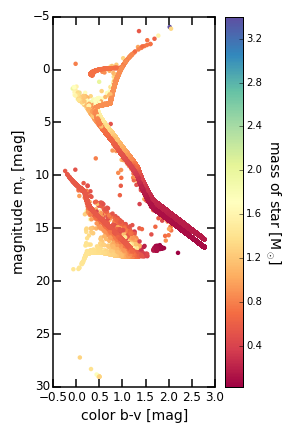
\includegraphics[width=\textwidth]{Plots/color_magnitude_diagram}
%\subsection{Orbits \& actions}
\par An orbit is a path a unperturbed, collisionless tracer particle (e.g. a star) will move along in a gravitational potential. Orbits contain information about the gravitational potential generated by the mass distribution of a system in their position and velocity coordinates following Newtons 2nd law. Orbit \acp{DF} describe which orbits are populated by how many tracers. From the orbit distribution function together with the overall potential we can draw inferences about the structure and evolution history of the system. 
\par Historically observations of orbits enabled discoveries or confirmed them: 
\begin{itemize}
\item Seen from the earth Mars' position moves over the sky as a loop called epicycle. That implies that the earth is not the centre of the universe! \citep[p.3]{2006ima..book.....C}
\item Neptune/Uranus \color{red} noch mal nachlesen \color{black}
\item From rotation curves of galaxies we see that stars move faster than what expected by the presence of only the mass of luminous matter. There has to be more matter interacting via gravitational forces. This has led to the theory of dark matter. (Rubin 1980)
\item Mercury's orbit differs hugely from calculated Kepler orbit. This is because of its migrating pericentre. Due to the proximity to the sun gravitational forces are so strong that we need to apply general relativity.
\item The \ac{SMBH} Sagittarius A*  was detected by observations of the orbits around the black hole and resulting mass calculations. \citep[p.923]{2006ima..book.....C} 
\end{itemize}
\par Some examples for orbit \acp{DF} are spiral galaxies where stars of different components (thin disc, thick disc, bulge, halo) are on different orbits (dynamical distinct) and have different metallicities (chemical distinct).
\\\par Actions are integrals of motion and are the distinct description of orbits. They are constant with time. Known for a long time they are extremly difficult to calculate. Actions of our solar system can be calculated more easily since the potential is a Kepler potential. With nowadays supercomputers it is finally possible to compute actions of more complex and less explored systems.
\color{green} how to describe orbits \\ idea 1 (x(t),v(t)) pretty complicated time evolution in 6 coordinates. idea 2 take quantities which are constant with time so called integrals of motions \\ beste set von integrals of motions are actions good to interpret \color{black}
\\\par In this thesis we wish to test the feasibility of the analysis of the action/orbit space in \acp{GC} and test whether it could be possible to predict  signatures of \acp{IMBH}. This will be done by "translating" the traditional phase-space into orbit space, exploiting the potential and the \(\vec{x}\) and \(\vec{v}\) vectors. Although this type of information (6-D info) is not currently available for Galactic \acp{GC} we are motivated by the growing amount of photometric and kinematic data that are already able to deliver a 5-D info (2D spatial info and 3D kinematic info), in particular the high accuracy \ac{HST} proper motions and the upcoming GAIA data. We will limit our analysis to \ac{GC} simulations with and without \acp{IMBH} to explore our new approach. The thesis is structural in to parts: first we familiarize with a phase space analysis of the simulations and we will focus in how to study the orbits and extract predictions of the presence of an \ac{IMBH}.





\newpage
\section{Method \& Theory}\label{method_theory}
\subsection{Stellar population in GC}\label{cmd_theory}
The typical stellar components of a \ac{GC} can be seen in a \ac{CMD}. In this \ac{CMD} the visual magnitude is plotted against the B-V color. It's color coded by the mass of the star. 
\begin{figure}[htbp]
\centering
	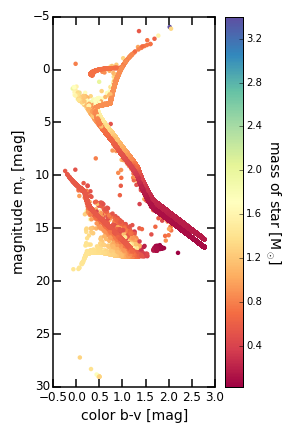
\includegraphics[width=0.5\textwidth]{Plots/color_magnitude_diagram.png}
	\caption{Color magnitude diagram of SIM 1.}
	\label{fig:cmd}
\end{figure}
A star's position can be interpreted as its evolution stage. Most of the stars are set in the main sequence. They fusion hydrogen in their cores. There are two main sequence lines one upon the other. These occur due to binary systems whose flux is given by the sum of the single fluxes of the single components, and therefore appear redder and more luminous. These binary systems represent about 5\% of the stars in the \ac{GC}. The position of the main sequence turn-off depends on the age of the system and therefore can be used as an indicator to determine the cluster's age. \color{red} explain isochrones \color{black} Bluewards of this turn off point following the trend of main sequence stars, there are so called "blue stragglers" which are remnants of stellar collisions or interacting binaries (B\&T p.628). Continuing from the turn off point there is the red giant branch consisting of stars still fusing hydrogen but only in a shell surrounding a degenerate helium core. They are inflated with a radius much higher than the main sequence stars but have a much lower temperature. These are the brightest stars of a \ac{GC}. On the upper part of the red giant branch lies the horizontal branch. Its stars burn helium in their core and hydrogen in a surrounding shell. In the lower left corner white dwarfs are located. They are stellar remnants which have burnt all of their resources. In a typical \ac{GC} dark stellar remnants like stellar black holes and neutron stars are present but not visualised in the \ac{CMD}. \color{red} nochmal über \ac{CMD} durchlesen\color{black} 
\subsection{Kinematic profiles of globular clusters}\label{kin_prof_theory}
\color{red} velocities are gauss distributed assumption \color{black}
Our investigations of \acp{GC} in phase space consists in analysing the spatial distribution of stars (density profiles) and the kinematic profiles(such as velocity dispersion and anisotropy profiles). First we test the sphericity of the \ac{GC}. Sphericity implies the usage of analytical methods that are very straight forward, especially for determing the potential of the globular cluster and then the actions in action space.\par \color{red} density profile \color{black} \par The velocity dispersion is the standard deviation of the mean velocity 
\begin{equation}
\sigma_i=\sqrt{\left\langle(v_i-\langle v_i\rangle)^2\right\rangle}=\sqrt{\left\langle v_i^2-\langle v_i\rangle^2\right\rangle} \qquad\qquad i=r,\theta,\phi.
\end{equation} For a spherical system it is best to calculate them in spherical coordinates \(r,\theta,\phi\) respectively \(v_r,v_{\theta},v_{\phi}\). If the \ac{GC} contains an \ac{IMBH} the velocity dispersion towards the centre is expected to increase. 
\par \color{red} what exactly describes anisotropy? \color{black} To quantify the anisotropy of the system we use the anisotropy parameter \(\beta\) 
\begin{equation}
\beta(r)\equiv1-\frac{\sigma_\theta ^2(r)+\sigma_\phi ^2(r)}{2\sigma_r ^2(r)}.
\end{equation} If \(\beta\) is positive the anisotropy is radial, if it is negative the anisotropy is tangential and if \(\beta\approx0\) then the system is isotropic.
\subsection{Density \& potential}\label{dens_pot_theory}
\subsection{Integrals of motion}\label{int_of_motion_theory}
\subsection{Orbits \& orbit integration}\label{orbit_theory}
\color{red} how does the orbit in a spherical potential look\\include effective potential\\ \color{black}
In a dynamical system the mass distribution is described by the form of theoretically existent orbits (\(\vec{x}(t),\vec{v}(t))\). Position and velocity are linked with six coordinates and contain all information about the potential. With Newton's 2nd law we get the connection between potential \(\Phi(\vec{r})\)and acceleration \(\vec{a}\) which is \[\vec{F}(\vec{r})=-\nabla\Phi(\vec{r})=m\cdot\vec{a}.\] Since the system is spherically potential and force only depend on the distance from the centre r. The potential can be derived from the Poisson's equation \begin{equation}
\Delta\Phi(r)=4\pi G \rho(r)
\end{equation}
with the density \(\rho\) depending only on the distance as well. Due to the spherical symmetry the potential can be calculated by 
\begin{equation}
\Phi(r)=-\frac{G}{r}\int_0^r{\mathrm{d}M(r')}-G\int_r^{\infty}{\frac{\mathrm{d}M(r')}{r'}}=-4\pi G\left[\frac{1}{r}\int_0^r\mathrm{d}r'r'^2\rho(r')+\int_r^{\infty}\mathrm{d}r'r'\rho(r')\right]
\end{equation} (Binney \& Tremaine eq. 2.28). We calculate the density by binning the masses on logarithmic equally distributed shells \color{red} write density formula? \color{black} and solve the integrals of the Poisson's equation numerically by using the Gauss-Legendre quadrature \[\int_a^b f(x)dx = \frac{b-a}{2}\sum_{i=1}^n w_i f\left(\frac{b-a}{2}x_i+\frac{a+b}{2}\right)\] where the points \(x_i\) and the weights \(w_i\) are derived from the Legendre polynomials.\\ Since the orbit is described by position and velocity at each time step we use the numerical leapfrog method which is a second-order time reversible integrator. \(X_i\) and \(v_i\) are calculated by 
\begin{align*}
x_{i+1}=x_i+v_i\Delta t+\frac{a_i(x_i)}{2}\Delta t^2 \\
v_{i+1}=v_i+\frac{a(x_{i+1})+a(x_i)}{2}\Delta t.
\end{align*}

\color{red} gcs are collisional clusters but we assume them as collisionless \\ time evolution of actions \color{black}


\subsection{Actions}
Stars in spherical symmetric potential are fully described by their actions \begin{equation}
J_i=\frac{1}{2\pi}\oint_{\gamma_i}\vec{p}\cdot d\vec{q} \qquad\qquad i=r,\theta,\phi
\end{equation} which are used as coordinates in action space
These actions are integrals of motion. For most potentials actions can't be described analytically. The actions of a spherical system are derived from angular momentum, energy and potential. Only the potential is depending in r. Energy and angular momentum as well as resulting actions are constant over time and orbit. The azimuthal action J\(_\phi\) and the latitudinal action J\(_\theta\) can be evaluated simply. To calculate the radial action J\(_r\) we have to solve an integral numerically. Actions of a spherical potential are found to be \begin{align}
J_\phi=L_z, \\ J_\theta=L-|L_z|, \\ J_r=\frac{1}{\pi} \int_{r_{min}}^{r_{max}} \mathrm{d}r \sqrt{2E-2\Phi(r)-\frac{L^2}{r^2}}.
\end{align}\color{red} Should I write down the derivation of the actions (B\&T p.220) or just the results (B\&T p.221, 3.221,3.223,3.224)?\color{black} \\ The pericenter \(r_{min}\) and the apocenter \(r_{max}\) as well as the guiding star radius \(r_g\) can be found in the effective potential \begin{equation}
V_L(r)=V(r)+\frac{L^2}{2mr^2}.\  \color{red} \mathrm{m\ should\ be\ left\ out\ right?} \color{black}
\end{equation} \color{red} Bartelman Theo 1 Skript p59 formula 6.27. \\ \color{black} In the peri- and apocenter the effective potential equals the total energy since the stars do not have any kinetic energy there. That results in following function which is to solve: \[\left(\frac{1}{r}\right)^2+\frac{2\cdot (\Phi-E)}{L^2}=0.\] \\ The guiding star radius is the distance at which a star with given total angular momentum would have a circular orbit. This is at the minimum of the effective potential. To get \(r_g\) we have to solve \[r\sqrt{r\frac{\partial\Phi}{\partial r}}-|L|=0\] where \(\sqrt{r\frac{\partial\Phi}{\partial r}}=v_{circ}\) is the circular velocity. This distance is used to have a better comparison of the actions since in the snapshot the stars are at a random position on their orbit.

\color{red} plot v\_eff plot from barthelman skript? \color{black}

\newpage
\section{Analysis}

\subsection{Description of the simulation}
\begin{table}[htbp]
\centering
\begin{tabular}{ c | c | c | c | c }
name of the simulation & \# of patches & total mass [M\(_\odot\)]& \makecell{mass of the \\ \ac{IMBH} [M\(_\odot\)]}& r\(_\mathrm{m}\) [pc]\\
\hline			
  SIM 1 - IMBH & 1026735 & 308533.2 & 10102 & 4.13 \\
  SIM 2 - IMBH & 1079376& 326253.4 & 8902.3 & 3.58\\
  SIM 3 - NOIMBH & 468627& 172671.3& 0 & 7.89\\
  SIM 4 - NOIMBH & 1851556& 669844.3& 0 & 5.41\\

\end{tabular}
\caption{Overview of the data of the simulations.\color{red} Question @ Paolo: Should \# of patches include IMBH? \color{black}}
\end{table}

\color{red}where simulation comes from and what it is \& description of output \color{black}\\
\\
To get a familiar with the simulation we first have a look at the scatter plot of the star positions.
\begin{figure}[htbp] 
\centering
\begin{subfigure}{0.9\textwidth}
	\centering
  	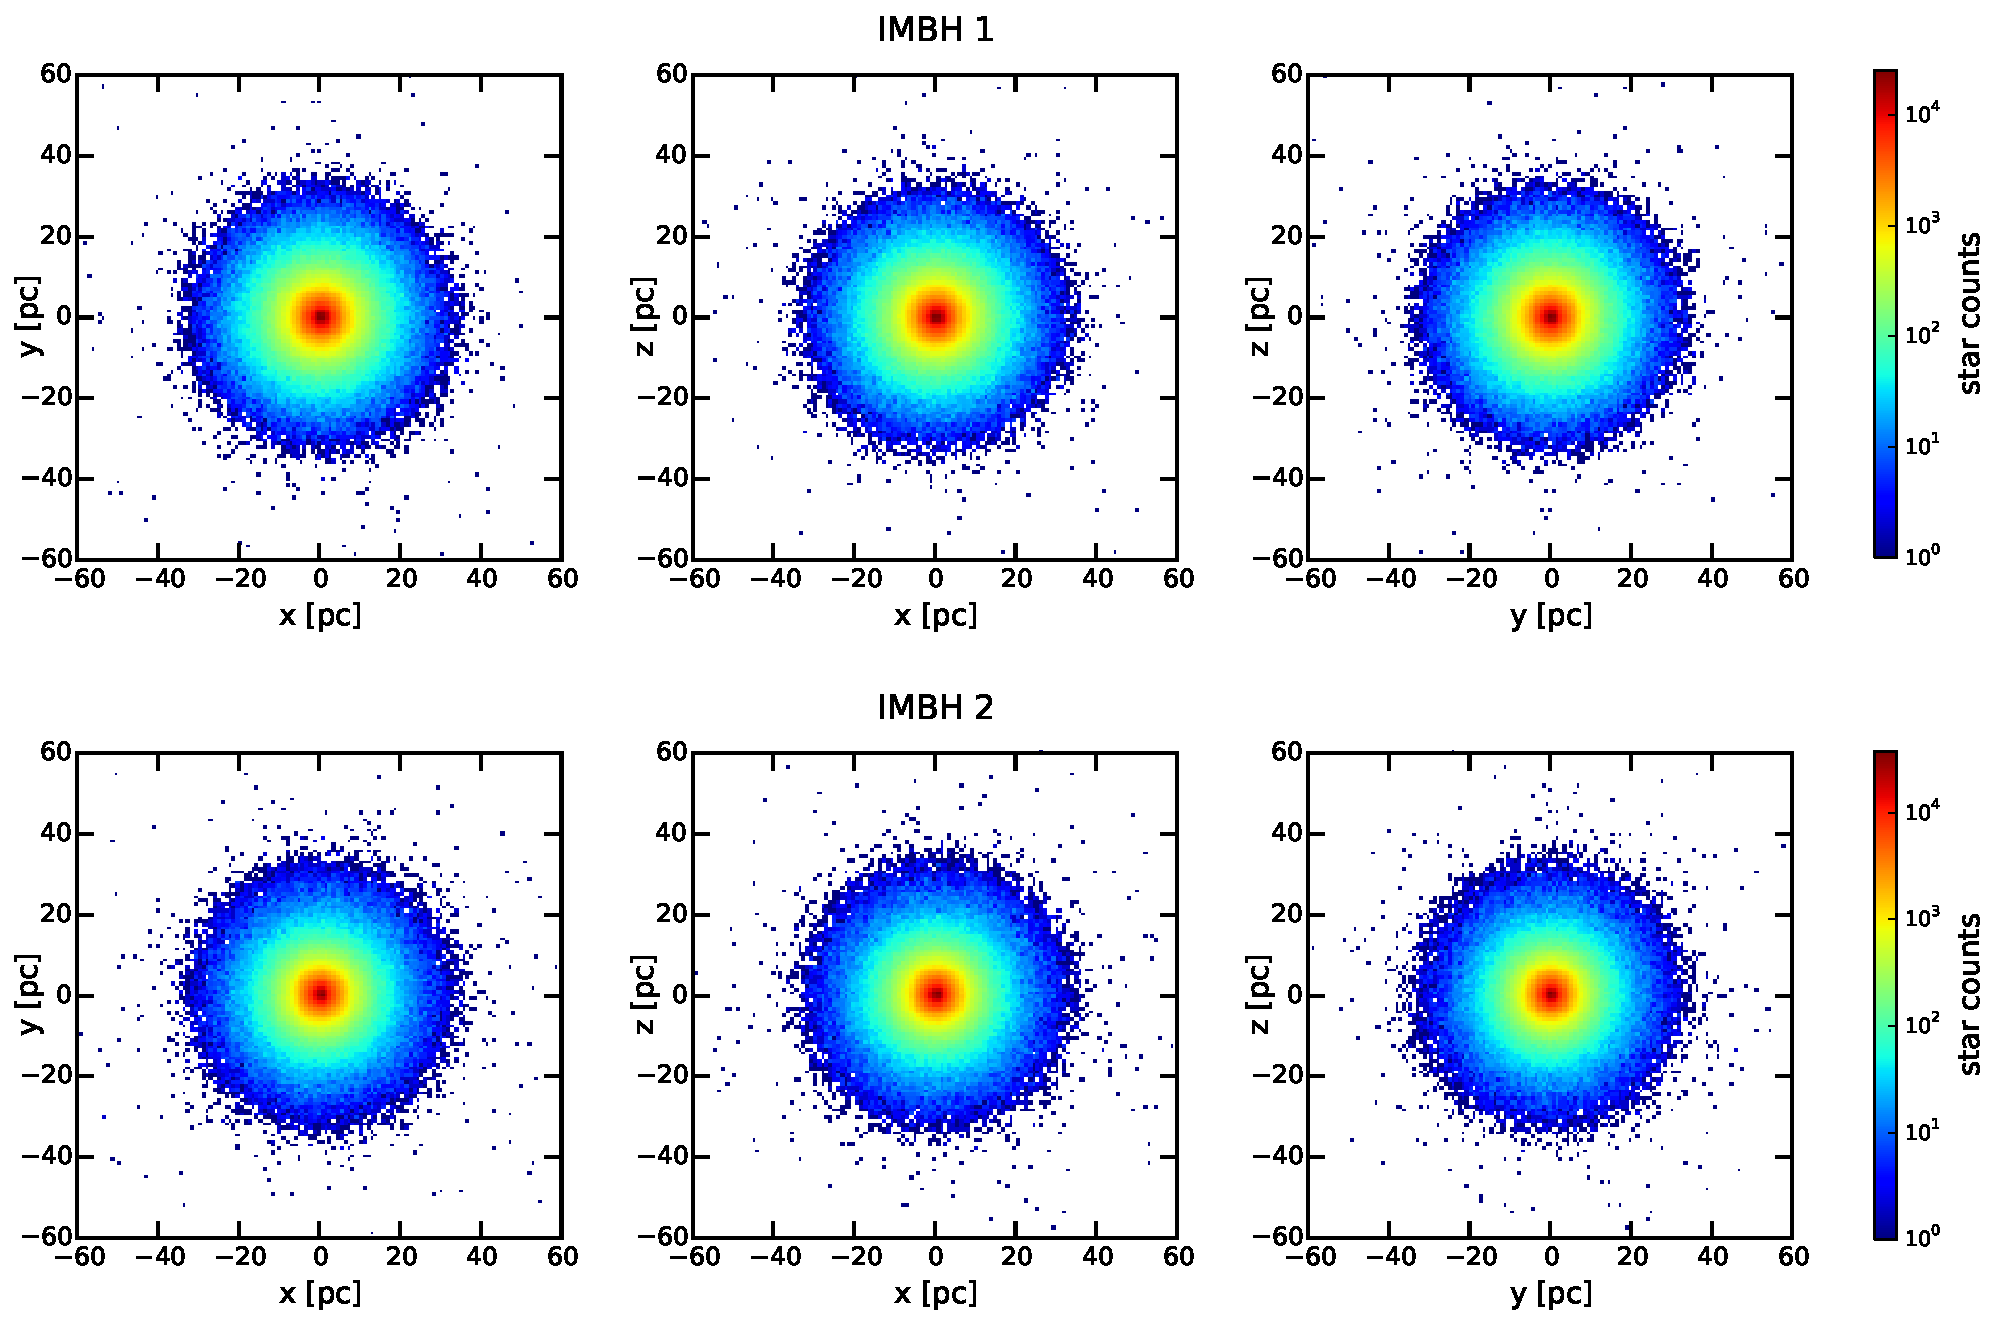
\includegraphics[width=\textwidth]{Plots/position_scatter_plot_IMBH.pdf}
  	\caption{SIM 1. The \acp{GC} are spread until 100 pc with most of the stars located in the inner 40 pc.}
 	\label{fig:pos_scat_IMBH}
\end{subfigure}
\\
\begin{subfigure}{0.9\textwidth}
	\centering
  	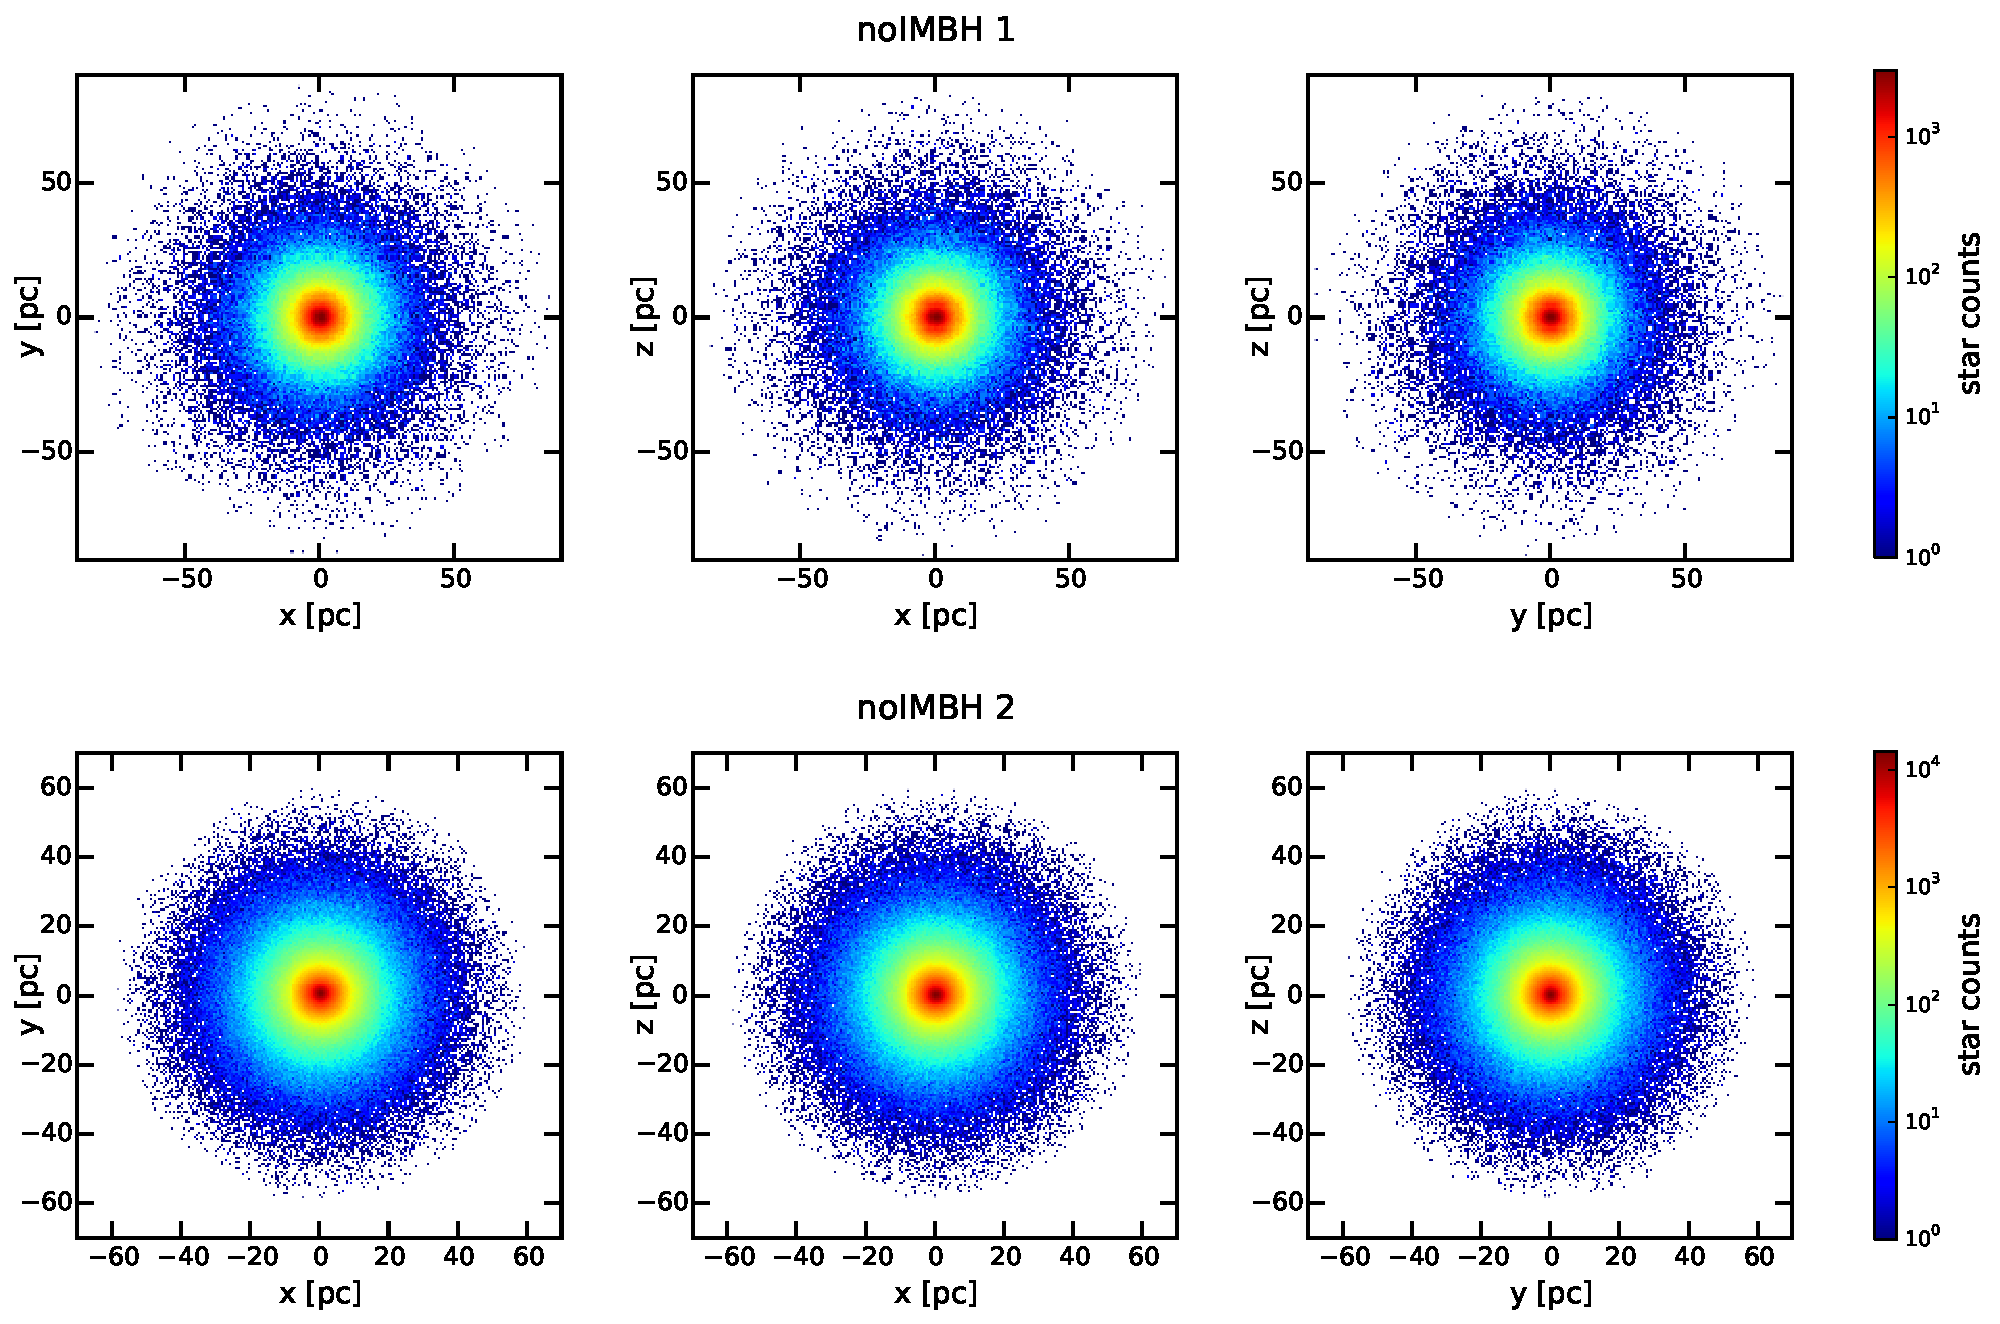
\includegraphics[width=\textwidth]{Plots/position_scatter_plot_noIMBH.pdf}
  	\caption{SIM 3. The \ac{GC} is spread until 90 pc (SIM3) and until 60 pc (SIM4).}
 	\label{fig:pos_scat_noIMBH}
\end{subfigure}

\caption{Position scatter plots. The stars are distributed spherically with most of the stars in the inner part. The stars of the \acp{GC} with \ac{IMBH} are less spread in the outer parts despite very few which are far outside. In the \acp{GC} without \ac{IMBH} the stars in the outer part are less accumulated but the furthermost stars still in the main sphere.}
\label{fig:position_scatter}
\end{figure}

\begin{figure}[htbp] 
\centering
\begin{subfigure}{0.95\textwidth}
	\centering
  	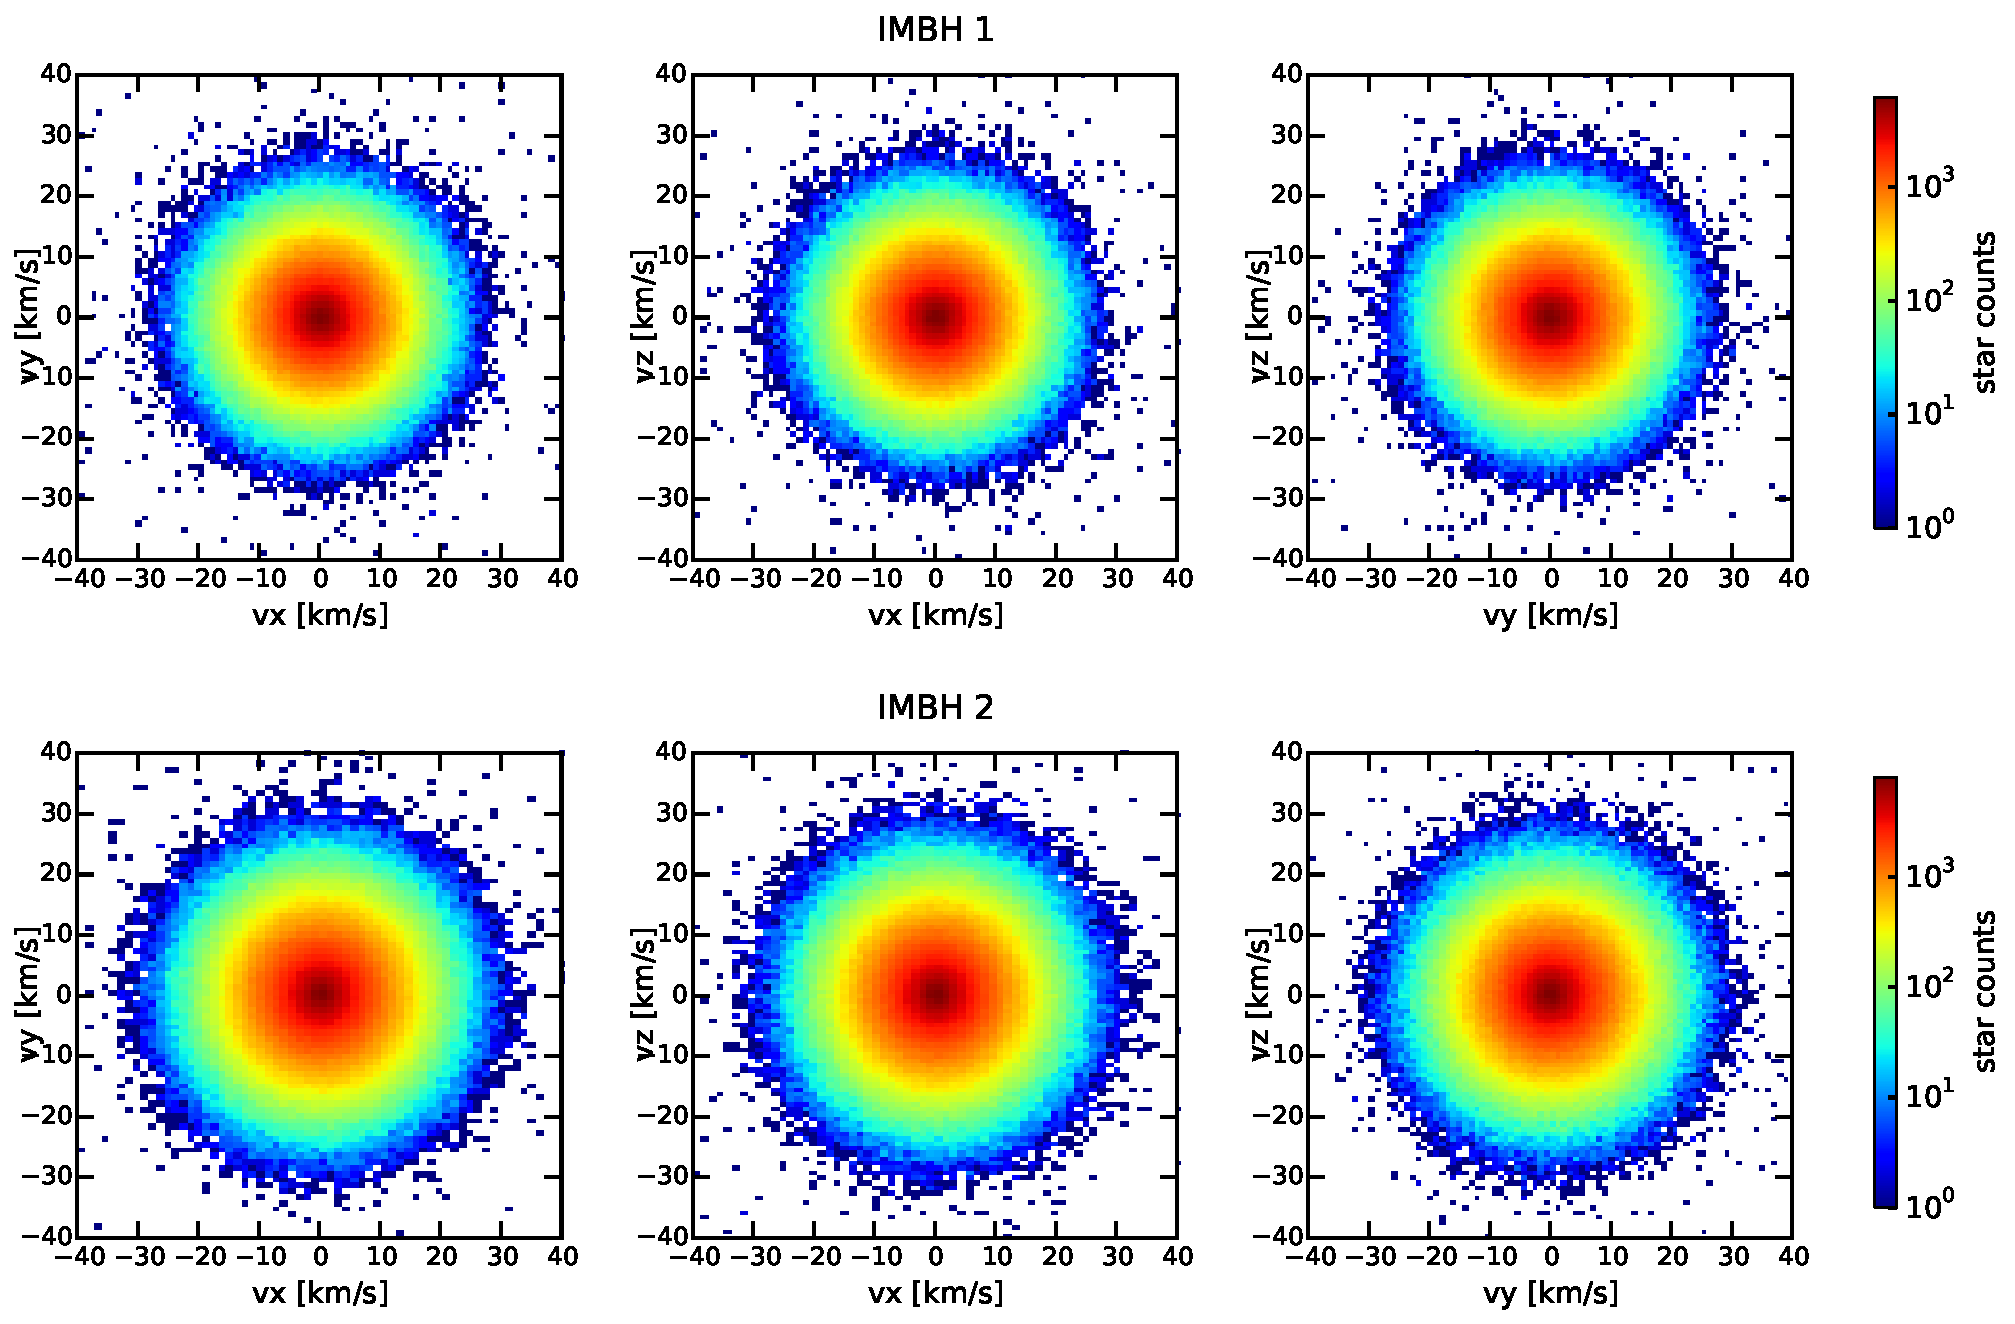
\includegraphics[width=\textwidth]{Plots/velocity_scatter_IMBH.pdf}
  	\caption{SIM 1. The stars' velocities are spread until 120 km/s with most of them reaching 30 km/s.}
 	\label{fig:vel_scat_IMBH}
\end{subfigure}
\\
\begin{subfigure}{0.95\textwidth}
	\centering
  	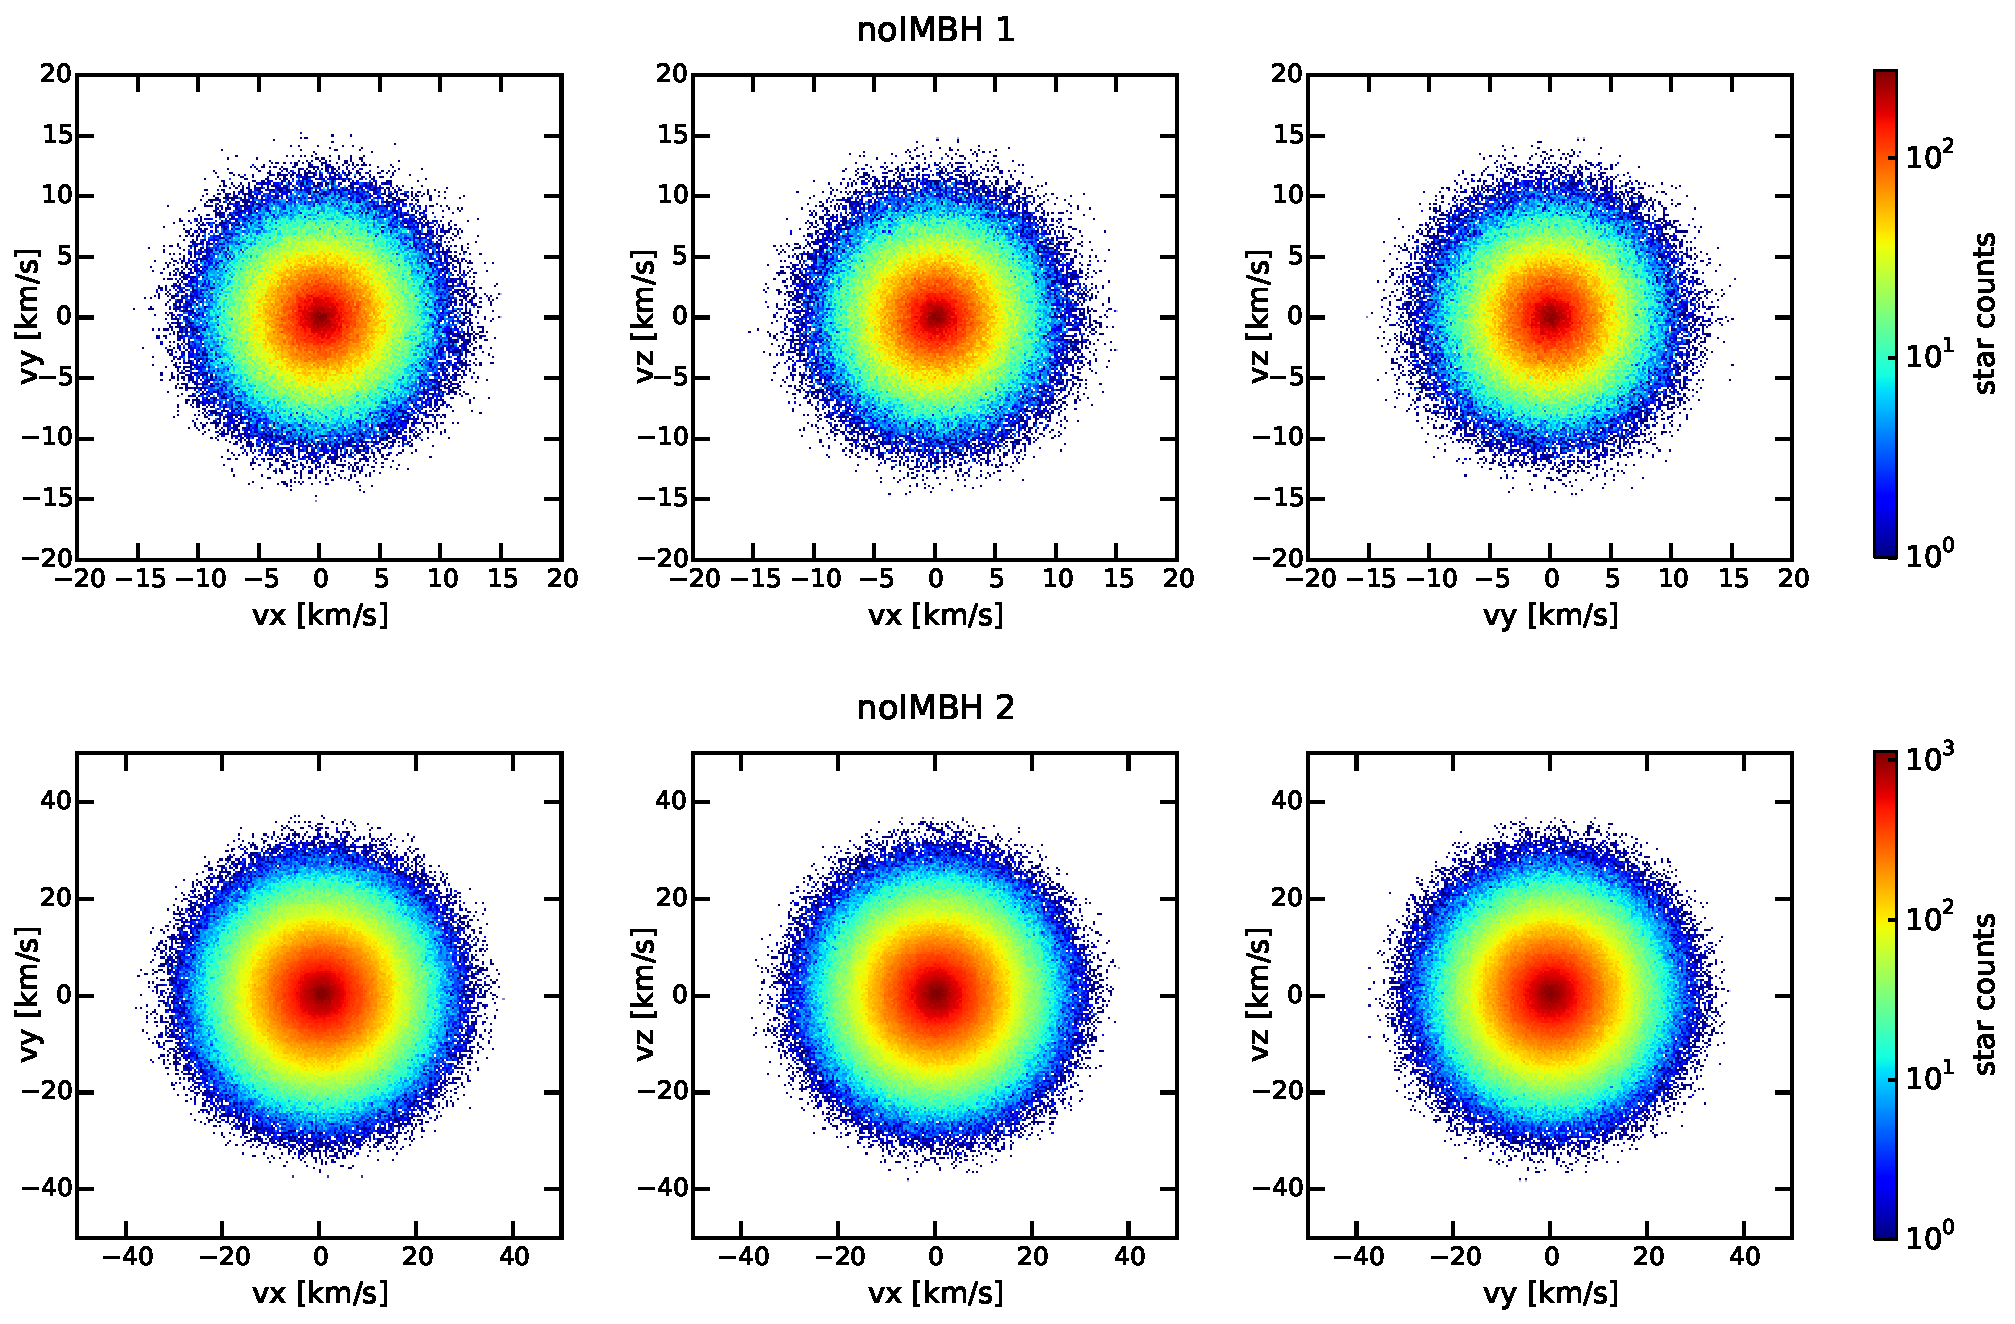
\includegraphics[width=\textwidth]{Plots/velocity_scatter_noIMBH.pdf}
  	\caption{SIM 3. The stars' velocities are spread until 15 km/s for SIM 3 whereas they spread until 40 km/s for SIM 4.}
 	\label{fig:vel_scat_noIMBH}
\end{subfigure}

\caption{Velocity scatter plots. The velocities are spherically distributed. Most of the stars have low or no velocity while a few have high velocities in different directions. Like the star distributions the velocity distributions of the \acp{GC} with \ac{IMBH} have some velocities outside the main sphere whereas the \acp{GC} without \ac{IMBH} contain all velocities inside the main shell.}
\label{fig:velocity_scatter}
\end{figure}
\color{red} include same plot with velocities!! \color{black}\\
As we said in section \ref{sec2.1} it is important to test the sphericity of a system. We will do this by splitting the \ac{GC} into octants and compare their mass \color{red} or number since we will introduce mass density plots only later \color{black} density \color{red} mass density sphericity plots\color{black}. As you see they're acceptable overlaying \color{red} within their errors. \color{black}
\\
As mentioned in \ref{sec1.2} the \ac{CMD} is showing a star's evolution stage dependend on its position. If you do not know age or metallicity of the system you can fit isochrones on the \ac{CMD}. Isochrones are curves of evolutionary stages of stars having the same age and metallicity but different masses. We plot several to our \ac{CMD} to determine which one fits best. This will give us the age and the metallicity of the system. 
\begin{figure}
	\centering
	\includegraphics[width=0.7\textwidth]{Plots/cmd_isochrones.pdf}
	\caption{Color magnitude diagram of SIM 1 overplotted with different isochrones. We recognize how we can determine the age based on the turn off point. This verifies the age and the metallicity of this \ac{GC} of 10 Gyr and 0.001.}
	\label{fig:cmd_isochrones}
\end{figure}


\subsection{Investigation in phase space}

First we will investigate the \ac{GC} in phase space for the set of simulations that w will use throughout this work. We will start with the velocity dispersion and the anisotropy parameter then we will have a density profile and from that get the potential. \color{red} for all 4 simulations or only for the first with IMBH? or with on plot containing two or all of them? \color{black}

\subsubsection{Velocity dispersion}
With (1) from section \ref{sec2.1} we can calculate the velocity dispersion for each coordinate \(r,\theta,\phi\). For every bin we take the same amount of stars and calculate the dispersion. To compare both simulations we plot the dispersion over the effective radius. The half mass radius of the simulation with \ac{IMBH} is 4.1pc and of the simulation without \ac{IMBH} it is 7.9pc. 
\begin{figure*}[htbp]
	\centering
	\begin{subfigure}{0.475\textwidth}
		\centering
		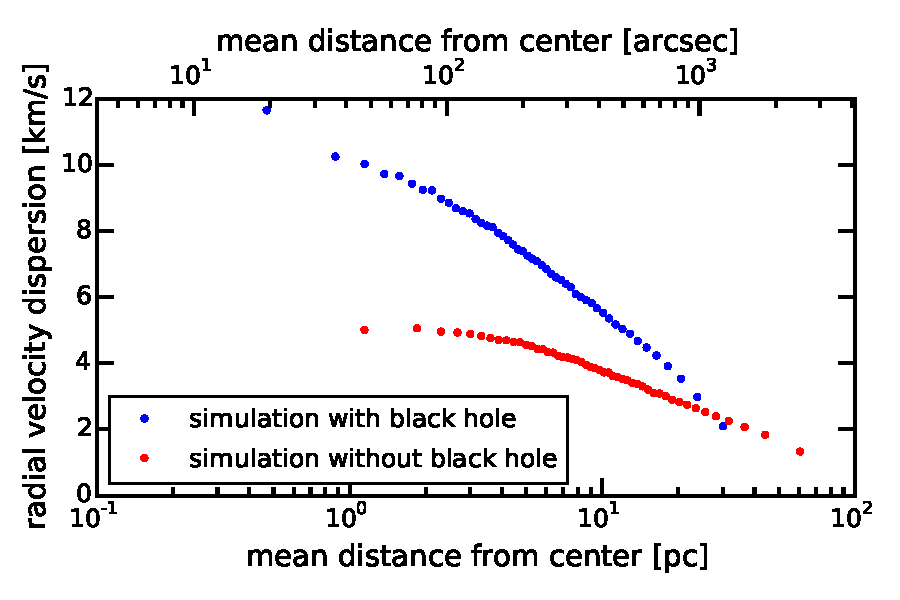
\includegraphics[width=\textwidth]{Plots/radial_velocity_dispersion.pdf}
		\caption{Radial velocity dispersions}
		\label{[fig:radial_vel_disp]}
	\end{subfigure}
	\hfill
	\begin{subfigure}{0.475\textwidth}
		\centering
		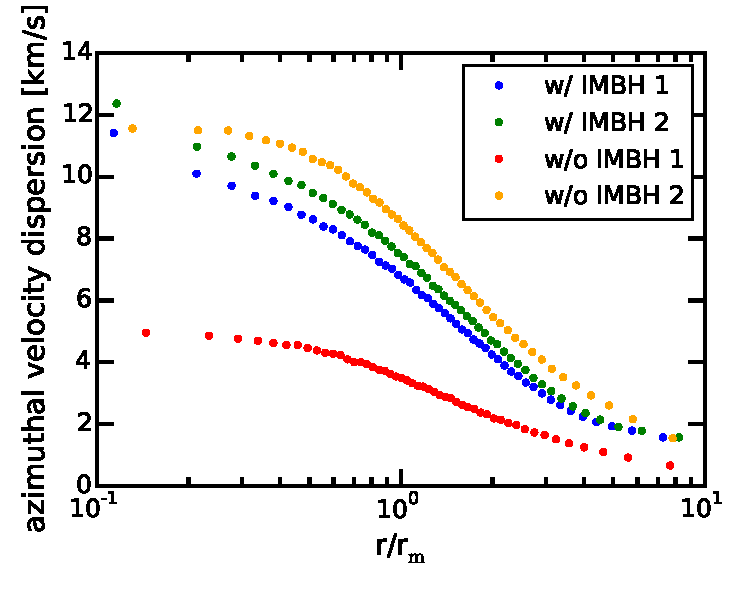
\includegraphics[width=\textwidth]{Plots/azimuthal_velocity_dispersion.pdf}
		\caption{Azimuthal velocity dispersions}
		\label{[fig:azimuthal_vel_disp]}
	\end{subfigure}
	\vskip\baselineskip
	\begin{subfigure}{0.475\textwidth}
		\centering
		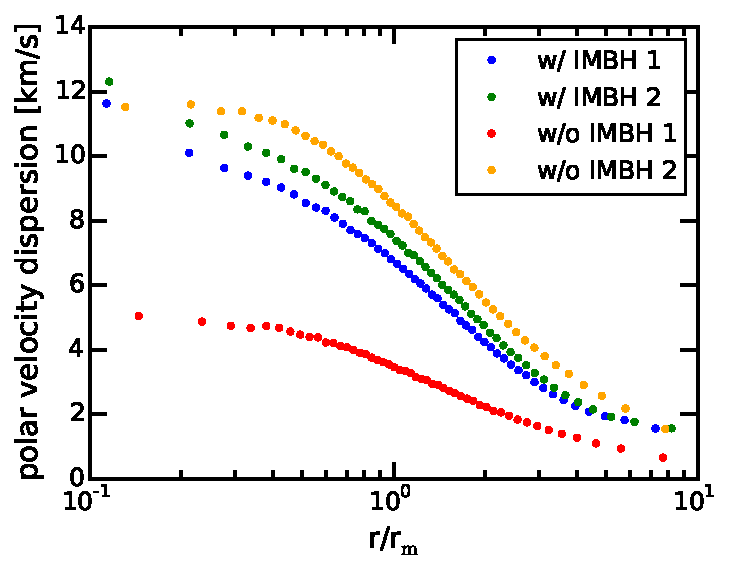
\includegraphics[width=\textwidth]{Plots/polar_velocity_dispersion.pdf}
		\caption{Polar velocity dispersions}
		\label{[fig:polar_vel_disp]}
	\end{subfigure}


	\caption{Velocity dispersion profiles as a function of the radius in units of the effective radius \(\mathrm{r_{eff}}\). They are binned in a way that each bin contains the same amount of stars. We can see that the velocity dispersion of the simulation with \ac{IMBH} rises towards the centre whereas the simulation without \ac{IMBH} exhibits a cored profile.}
\end{figure*}
As expected there is a rise in the centre for the simulation with \ac{IMBH}. This is due the high gravitational potential of the \ac{IMBH} which disturbs the dynamics of close stars. 


\subsubsection{Anisotropy}
Anisotropy can be calculated from (2) in \ref{sec2.1}. It is binned the same way as for the velocity dispersion and again dependent on the effective radii.
\begin{figure}
	\centering
	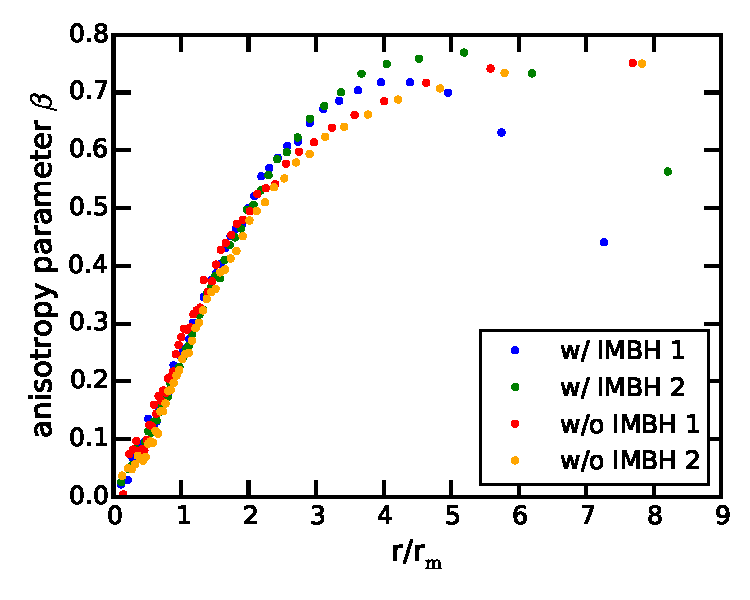
\includegraphics[width=0.475\textwidth]{Plots/anisotropy_parameter_beta.pdf}
	\caption{Anisotropy parameter \(\beta\). All simulations are radial anisotropic. The simulations with \acp{IMBH} have a peak at 4 and 5 effective radii where they are most radial anisotropic. The other simulations are rising until the end. The far more outside a star is the higher its radial anisotropy is. Within the first two effective radii all seem to have the same course.}
	\label{fig:anisotropy_param}
\end{figure}
In the center of both \acp{GC} there is nearly the same anisotropy. Both are positive and rising. That means the systems are radial anisotropic. The \ac{GC} with \ac{IMBH} is most radial anisotropic in its center at about 4 effective radii. The other \ac{GC} is becoming more radial anisotropic the more far from the centre it is.

\subsubsection{Density profile}
The density profile shows the density of the system over its radius. The bins are chosen so that the radii are equidistant on a logarithmic scale and that they are at least 100 stars per bin to have a reliable stochastic. Outside of the cluster the density is set to 0. In the innermost part the density is set to be as the innermost point.
plots\\
\begin{figure}
	\centering
	\begin{subfigure}{0.475\textwidth}
		\centering
		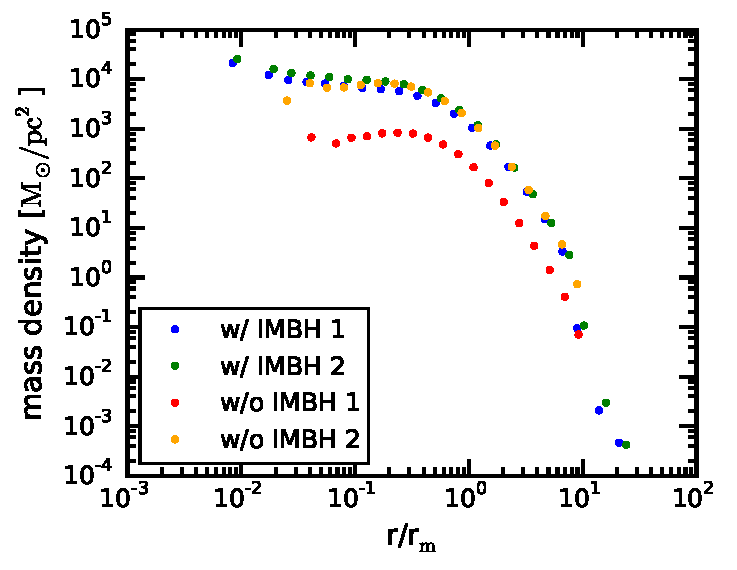
\includegraphics[width=\textwidth]{Plots/density_profiles.pdf}
		\caption{Mass density profiles of all four simulations.}
		\label{mass_dens_points}
	\end{subfigure}
	\hfill
	\begin{subfigure}{0.475\textwidth}
		\centering
		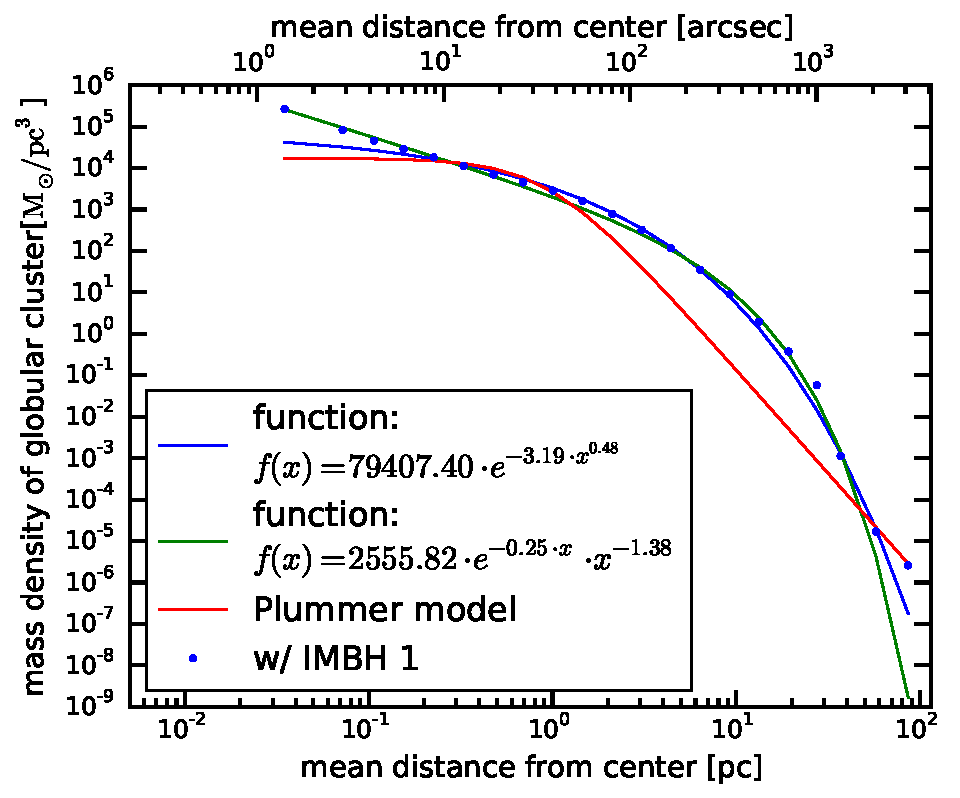
\includegraphics[width=\textwidth]{Plots/density_prof_analytic.pdf}
		\caption{Analytically fitted mass density profile of SIM 1.}
		\label{mass_dens_ana}
	\end{subfigure}
	\vskip\baselineskip
	\begin{subfigure}{0.475\textwidth}
		\centering
		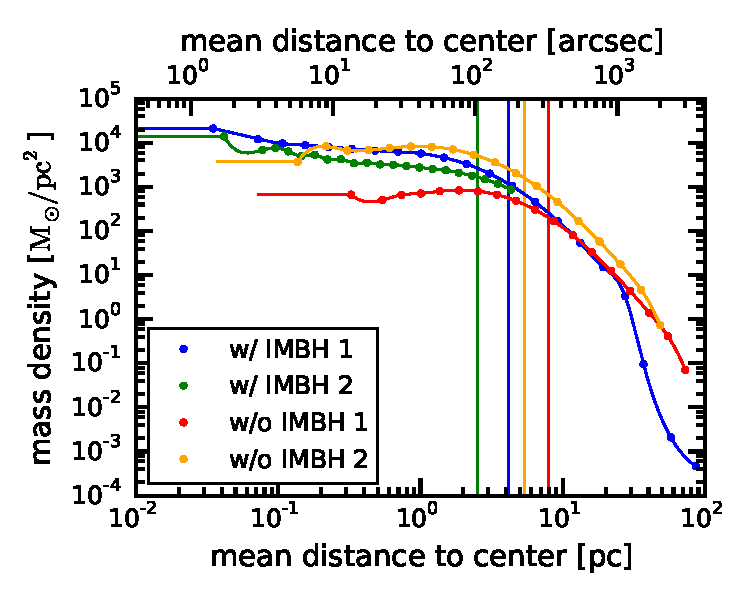
\includegraphics[width=\textwidth]{Plots/density_profiles_interpolated.pdf}
		\caption{Interpolated mass density profiles of SIM 1 and SIM 3.}
		\label{mass_dens_intpol}
	\end{subfigure}
	\caption{Mass density profiles. The density in \(\frac{M_{\odot}}{pc^2}\) is plotted against the effective radius. The density of the \ac{GC} with \ac{IMBH} is everywhere larger than the density of the \ac{GC} without \ac{IMBH}. In the centre there is a raise in the density of the \ac{GC} with \ac{IMBH} whereas the other \ac{GC} stays approximately on the same level. Both start decreasing at about 0.5 \(\mathrm{r_eff}\). We can see in \ref{mass_dens_intpol} that it is not simple to find an analytical function describing the density. Thats why we interpolate it in \ref{mass_dens_intpol}. Everything out of the \ac{GC} is set to 0 while the innerst density is set to be the value of the innermost point.}
	\label{fig:mass_density_profile}
\end{figure}

\subsubsection{Potential}
From the density profile we can compute the potential as described in \ref{dens_pot_theory}. It is composed by the potential given from the stars and if there is one the potential of the \ac{IMBH} expressed as Kepler potential.
\begin{figure}
	\centering
	\includegraphics[width=0.475\textwidth]{Plots/Pot.pdf}
	\caption{Potential of all \acp{GC}. SIM 1 and SIM 2 are nearly overlaying. They are the same simulation at different ages. The simulation lost 5 \% of it's stars with 10 \% of the total mass while the \ac{IMBH} gained 13 \%. The potential of the stars declines while the potential of the \ac{IMBH} rises so the potential stays the same. The \acp{GC} without \ac{IMBH} remain constant in the inner part (until 0.5 half mass radii) and decrease from the points where their densities decrease.}
\end{figure}


\subsection{Investigations of orbits in action space}
wilma class 
\subsubsection{Orbits \& actions}


\subsubsection{Integral of motions along orbits}

\newpage
\section{Results \& Discussion}


\subsection{Signatures of \acp{IMBH} in action space}\label{results}

\begin{figure}[htbp]
\centering
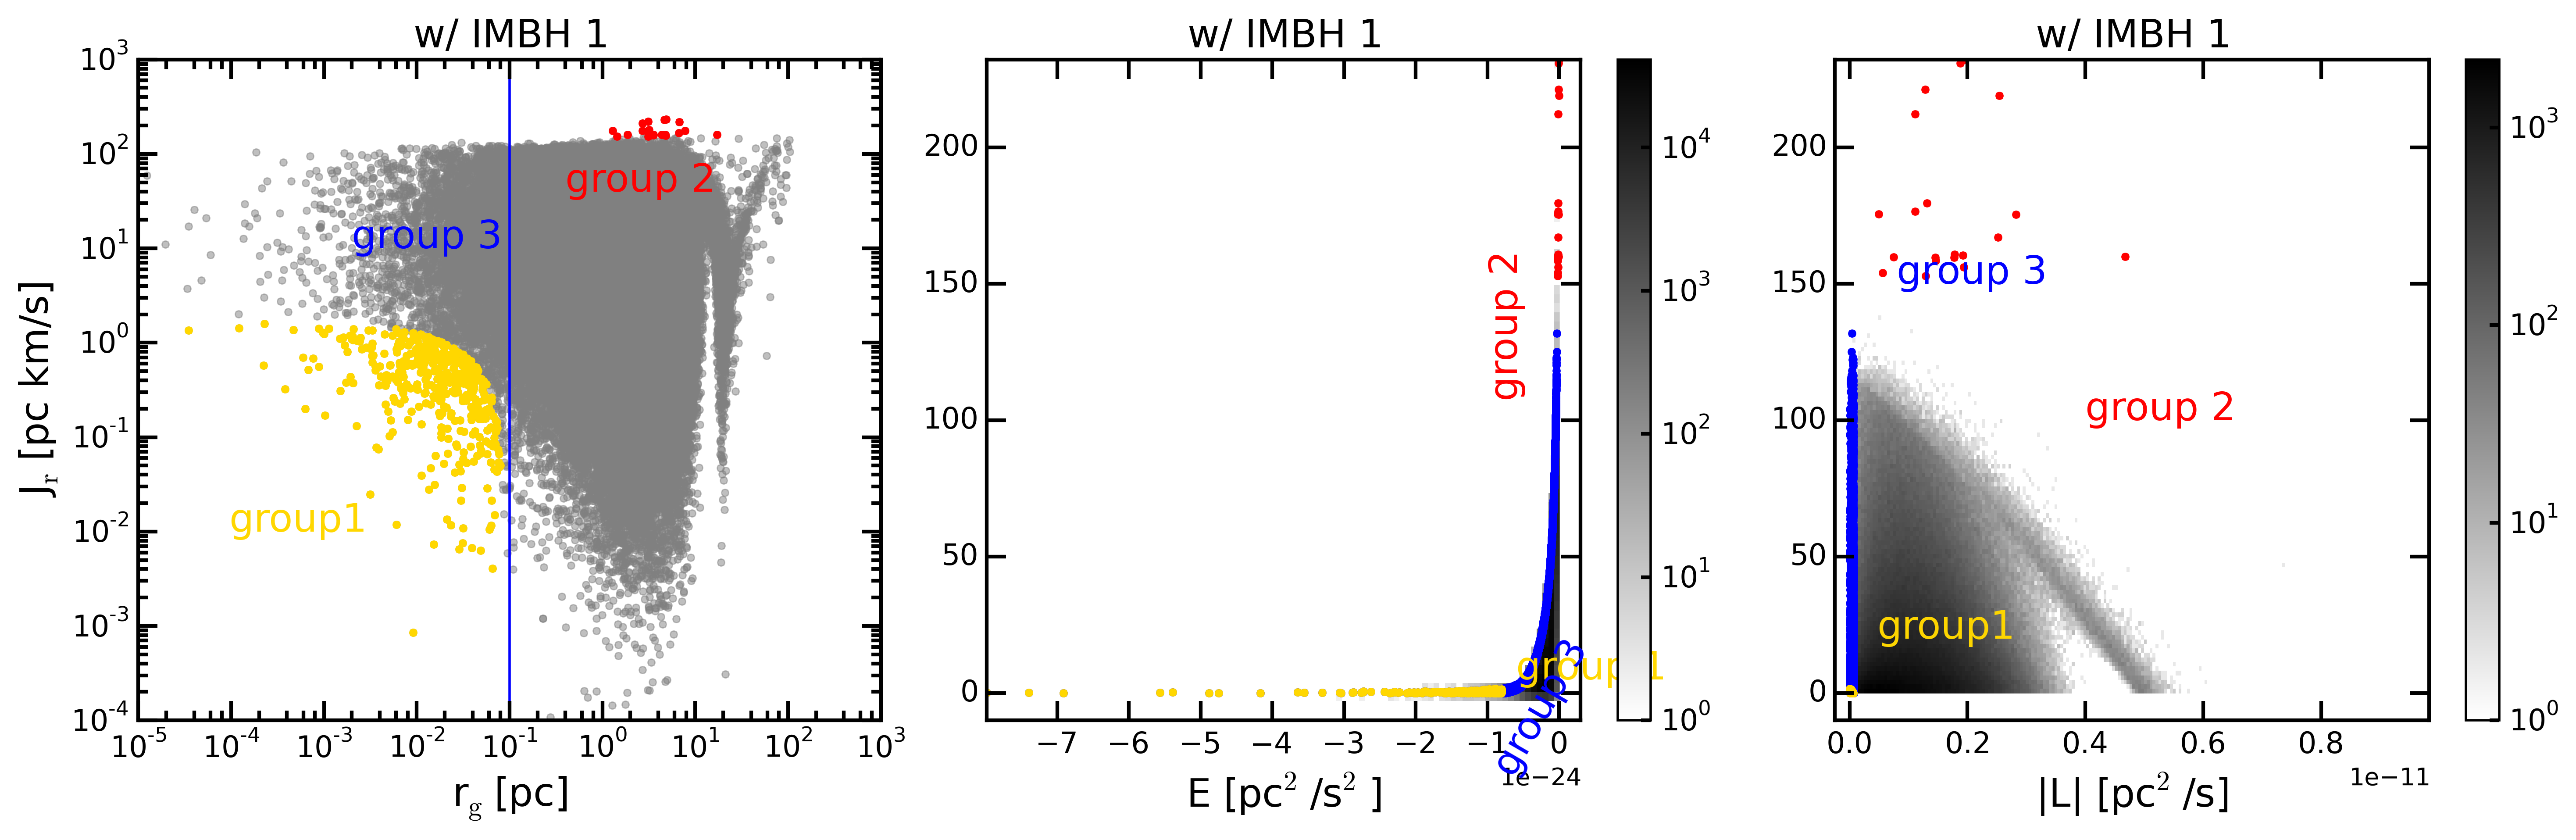
\includegraphics[width=\textwidth]{Plots/J_r_compare_plot.png}
\caption{Radial action over different values.}
\label{fig:J_r_compare}
\end{figure}

\subsection{Discussion \& future perspectives}
In summary we can say that we found clearly evidence of the \ac{IMBH} in the radial actions. To get there we made some simplified assumptions which should be investigated more precisely in an extended work. The density is the basis of our approach of the actions. Since we didn't find an analytical function we interpolated the binned densities and set the central density equal to the innermost density bin. Another attempt to get the density could be done by modelling Multi-Gaussian Expansion to the graph. But for this thesis we see the interpolation as sufficient since tests with some different densities do not destroy the figures of section \ref{results}. \par Additional inaccuracy of the results rises due to different simulations for \acp{GC} with and without \ac{IMBH}. Since they have different initial conditions and conditions throughout the simulating process we can not compare them directly. Especially the radial actions can not be compared since they are mass dependent. We see the differences directly in the scatter plots (figures \ref{fig:position_scatter} and \ref{fig:velocity_scatter}) and in the anisotropy due to different truncation prescriptions. In further investigations we should consider using simulations with same conditions despite only the absence of an \ac{IMBH} in one of the simulations. \par Some physical assumptions have been that actions stay totally constant over time or rather that we have only looked at them at the time of the snapshot (despite a few stars for which we integrated the orbit and have looked at the time evolution of their integrals of orbits). Changing integrals of motion go along with changing orbits which could have some numerical fluctuations especially near the \ac{IMBH}. \par Another assumption is that we use specific values if not said else. That means we divide all values by the mass of the stars. We see in fig \ref{fig:L_J_r_hist} that there can be distortion due to that. Further work can investigate the mass dependency of the integrals of motion. \par If all these points are applied to this method we should think of a way to apply this approach to observational-like data. The main difference is that at this moment there is no possibility to get the masses of the stars of \acp{GC} and therefore we can not derive the potential which is essential for this method. 





\newpage
%\section{Conclusion}
%\newpage 
\section{Acronyms}

\begin{acronym}[SMBH]
	\acro{CMD}{color magnitude diagram}
	\acro{COM}{centre of mass}
	\acro{DF}{distribution function}
	\acro{GC}{globular cluster}
	\acro{v-GC}{Globular clusters}
	\acro{HST}{Hubble Space Telescope}
	\acro{IMBH}{intermediate mass black hole}
	\acro{MW}{Milky Way}
	\acro{SMBH}{super massive black hole}
	\acro{SSP}{single stellar population}
\end{acronym}
\newpage
\bibliography{Literatur}
\addcontentsline{toc}{part}{Bibliography}



\end{document}